% !TEX root = main.tex
%%%%%%%%%%%%%%%%%%%%%%%%%%%%%%%%%%%%%%%%%%%%%%%%%%%%%%%%%%%%%%%%%%%%%%%%%%%%%%%%
% Introduction
%%%%%%%%%%%%%%%%%%%%%%%%%%%%%%%%%%%%%%%%%%%%%%%%%%%%%%%%%%%%%%%%%%%%%%%%%%%%%%%%
\section{Introduction}
\label{section:introduction}
The Cray XK7 Titan supercomputer~\cite{olcf:titan} was the \#1 system
in the world for a very long time~\cite{top500list}, and has remained
a critically important computer system through the end of its life in
the Summer of 2019. It defied scale with 18,688 individual compute
nodes and delivered tens of billions of computing hours to the
U.S. Department of Energy mission-critical programs for nearly 7
years.
 
From a realiability perspective, Titan was a very interesting
machine. Its operation was forced to execute three very significant
rework cycles, two on the mechanical assembly affecting the PCIe
connector from the GPU daughtercard to the motherboard, and one to
replace about 11,000 GPU assemblies because of a failing resistor on
their printed circuit board. We write primarily about the GPU
operation epoch that includes this last rework cycle. This epoch of
nearly 6 years includes Titan's most stable and failure free period
and contains the most reliable data on GPU operation.

\begin{figure*}[tb]
  \centering
  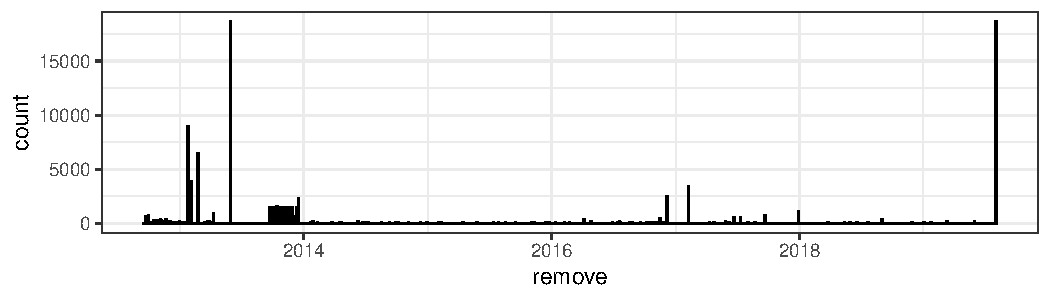
\includegraphics[width=\textwidth]{figs/chronology001.pdf}
  \caption{Volume of GPU swaps detected on Titan at individual
    inventories (narrow blue) and yealy sum totals for 2014 and later
    (wide gray) over its entire lifetime. High swap volumes prior to
    2014 reflect two major rework cycles on mechanical assembly issues
    at PCIe connectors that can be characterized as a break-in
    period. Our analysis in this paper excludes the break-in period
    and is focused on units in place by the end of 2013 or swapped in
    during the years that follow.}
  \label{fig:chronology}
\end{figure*}
Figure~\ref{fig:chronology} illustrates the chronology of the rework
cycles and stable periods as indicated by the number of GPU changes at
periodic inventories. The first two rework cycles before 2014
involving blade mechanical assembly can be characterized as a break-in
period on a new system that is first of its kind and pushes many
technological boundaries. The resulting field engineering as well as
data collection changes are responsible for the high GPU swap counts
before 2014. Late 2013 begins a very long period of high reliability
and stable operation with very few issues until about mid 2016, when
GPU failures begin to rise. This results in the final rework cycle,
replacing 11,000 GPUs throughout much of 2017. The peak at the end in
the figure is an artifact of turning off or ``removing'' all the
units as Titan is shut down and disassembled.

Finding the root cause for the 2016 failures took a great deal of
testing and involvement of materials science and microscopy
researchers. The failures were traced to a resistor on the GPU
circuit board (not the GPU chip iself). Throughout this paper, when we
refer to replacing the GPU, we refer to the entire circuitboard along
with its GPU chip.

Our analysis focuses on GPU boards that were installed in the second
rework cycle and later, essentially units installed near the beginning
of 2014 and later. Figure~\ref{fig:chronology} is the only one
involving data prior to 2014. All analyses and figures that follow use
only data from 2014 onward. We make the data as well as our analysis R
codes and Python codes to reproduce the graphics in this paper
publicly available (see, \cite[repository to be added in final
version]{repositoryreference,rcodes,pycodes}).  While the data is only
a 7 MB file, due to the size of Titan it represents over 100,000
collective years of GPU operation and may be the largest publicly
available GPU reliability data set. Our hope is that others will use
it for reliability and survival analysis research and go beyond the
results presented here.

We begin by describing related work in Sec.~\ref{section:related}. Our
data collection is described in Sec.~\ref{section:dataprep} and the
data cleaning, checking, and lifetime summarization process in
Sec.~\ref{section:dataclean}. A time between failures (TBF) analysis
is given in Sec.~\ref{section:tbf}. Survival analysis \rev{(SA)} based on
Kaplan-Meier modeling (KM) and Cox regression modeling (CR) of
relative hazard rates in various locations are in
Sec.~\ref{section:survival}. The goals of a TBF analysis and of
SA are different: TBF studies largely show GPU
reliability affects the machine, whereas SA studies largely how the
machine affects GPU reliability.  Finally, we discuss our main
conclusions and recommendations in Sec.~\ref{section:discussion}.
 


